\section{Implementation}
\subsection{General implementation}
	The basic simulation consists only of evaluating equations for every time step. The implementation can be found in the \textit{Hive.m} code, appendix \ref{chap:MATLAB_Hive}. Variable names are chosen so that they match \textit{Khoury et al.} \cite{khoury13} and chapter \ref{chap:basicModel} as close as possible.\\
	For the advanced model, the following hierarchy is used: The top level is the \textit{hive\_simulation.m} (\ref{chap:MATLAB_hive_simulation}) file, which sets up the whole simulation. Then it keeps track of data and iterates through days in the hive simulation and through seconds in the environment simulation. The \textit{Prop} class (\ref{chap:MATLAB_Base}) is an implicit struct which allows to plug in and change empirical data and simulation parameters. For the environment simulation, \textit{Bee} (\ref{chap:MATLAB_Bee}) is the class for agents, \textit{Hive} (\ref{chap:MATLAB_Hive}) for hives and \textit{World} (\ref{chap:MATLAB_World}) for the maps.\\
	The final report (simulation results) is stored as class \textit{Report} (\ref{chap:MATLAB_Report}) with an implicit struct, making data analysis easy and extendible.\\
	All important code files can be found in appendix \ref{chap:MATLAB_Code}.
	
\subsection{Map and flower patch quality}
	\label{chap:mapFlowerPatchQuality}
	
	The bees all navigate on a map with the hive in the middle of the map. Every pixel on the map equals to a patch of 100 m$^2$.\\
	
	\begin{figure}
		\centering
		\scalebox{.2}{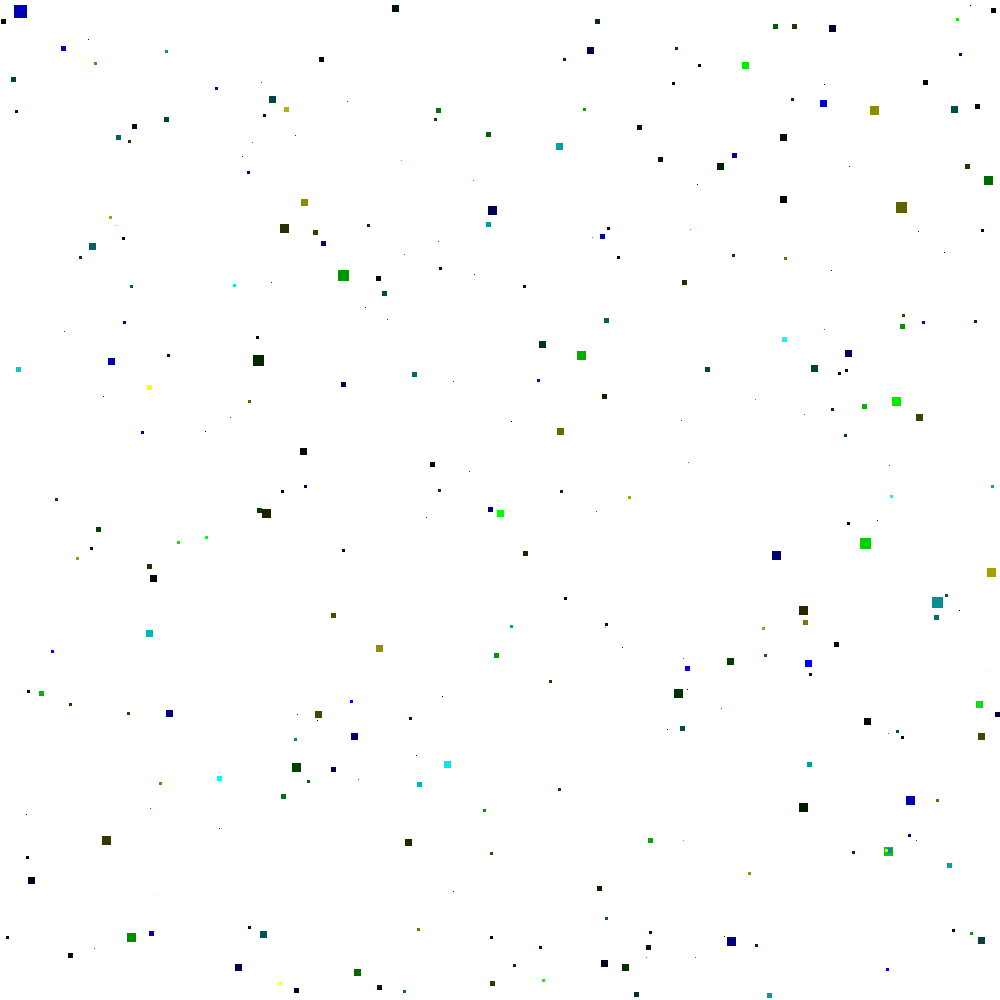
\includegraphics{data/equal_dist_normal_iv.png}}
		\caption{\textit{Example of an equal distributed flower patch, normal distributed quality map. Note that the encoding is given by Figure \ref{fig:hsvEncoding} but background black has been swapped out with white for better visibility.}}
		\label{fig:normeqMap}
	\end{figure}
	
	The map is encoded in HSV (fig. \ref{fig:hsvEncoding}). From the 360° color hue circle ($H_{HSV} \in \{0,1,\ldots,360\}$), always 60° are assigned to one integer type value $j \in \{0,\ldots,5\}$. Value 0 is used for empty space and values 1 to 3 for the three flower seasons/types we implemented. Values 4 and 5 are for future extensions such as smog/pesticide sources. More values can be gained by assigning less than 60° per type. The saturation $S_{HSV} \in [0,1]$ is always kept at 1. For the flower patch quality basis, the $V_{HSV} \in [0,1]$ component is used.\\
	
	To obtain the daily map for environment simulation, the normalized blooming indicator (see fig. \ref{fig:seasonalFlowers}) of each flower type $i \in \{1,2,3\}$ is separately multiplied with the $V_{HSV}$ value of the basis map where flower type $i$ occurs (see fig. \ref{fig:normeqMap}). As a result, some flowers don't appear on the map and those that appear get scaled in quality according to the daily situation (see fig. \ref{fig:modelOverview}). From the obtained scaled quality map, the bees now read the value $b_w$ when visiting a patch. This is the driving factor for forager distribution (see chapter \ref{chap:foragersDistribution}).
	
	\begin{figure}
		\centering
		\scalebox{.7}{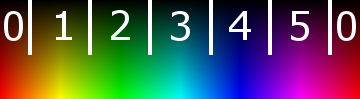
\includegraphics{data/hsv_encoding.png}}
		\caption{\textit{Map encoding in HSV.}}
		\label{fig:hsvEncoding}
	\end{figure}
	
	
\subsection{Scouts}
	\subsubsection{Random walk}
		Very little is known about the searching behaviour of scout bees \cite{seeley95}, p.~87f. \textit{T.D. Seeley} mentions that scouts fly low above the ground and inspect flowers they encounter during their flight. Naturally, the flight distance is limited. Considering this, a random walk is the most logical behaviour to simulate scout bees. The random walk is stopped when a scout encounters a new flower. Previously discovered flower patches are ignored by scouts, as bees mark already visited patches with the Nasonov pheromone \cite{winston91} p.~133ff.\\
		The random walk is preformed in following steps:
		\begin{itemize}
			\item The bee starts from the hive with an equally distributed random angle $\alpha \in [0, 2 \cdot \pi]$ (radian).
			\item After a number of time steps (we've chosen one time step, so 60 seconds), the angle $\alpha$ is changed by at most $r\cdot0.5$ (radical angle changes are not desired), where $r$ is a normal distributed random value.
			\item Between two angle changes, the scout bee flies with 7 m/s into the chosen direction.
			\item The path points are recorded at every angle change point. The distance passed is calculated and stored in a $L^2$ norm scalar.
		\end{itemize}
		
		The path a scout bee walks is recorded in a vector of $x$ and $y$ coordinates:
		\[\begin{pmatrix}
			x_0 & x_1 & \ldots & x_n \\ y_0 & y_1 & \ldots & y_n
		\end{pmatrix}\]
		where $\begin{pmatrix} x_0 \\ y_0 \end{pmatrix}$ are the hive coordinates and $\begin{pmatrix} x_n \\ y_n \end{pmatrix}$ are either the coordinates with maximum possible distance from the hive according to $L^2$ norm, or the coordinates of a flower patch.\\
		
		An example of such a random walk is given in Figure \ref{fig:randomWalk}.
		
		\label{chap:randomWalk}
		\begin{figure}
			\centering
			\scalebox{.75}{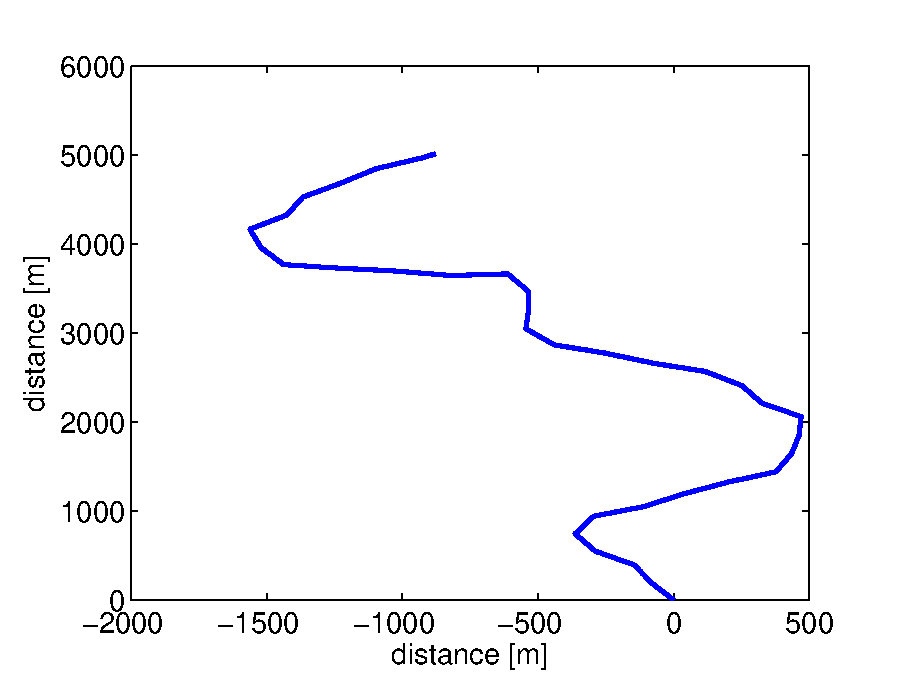
\includegraphics{data/random_walk.eps}}
			\caption{\textit{Example of a random walk executed by a scout bee.}}
			\label{fig:randomWalk}
		\end{figure}
		
	\subsubsection{Bresenham line algorithm}
		\label{chap:bresenhamAlgorithm}
		\begin{figure}
			\centering
			\scalebox{.75}{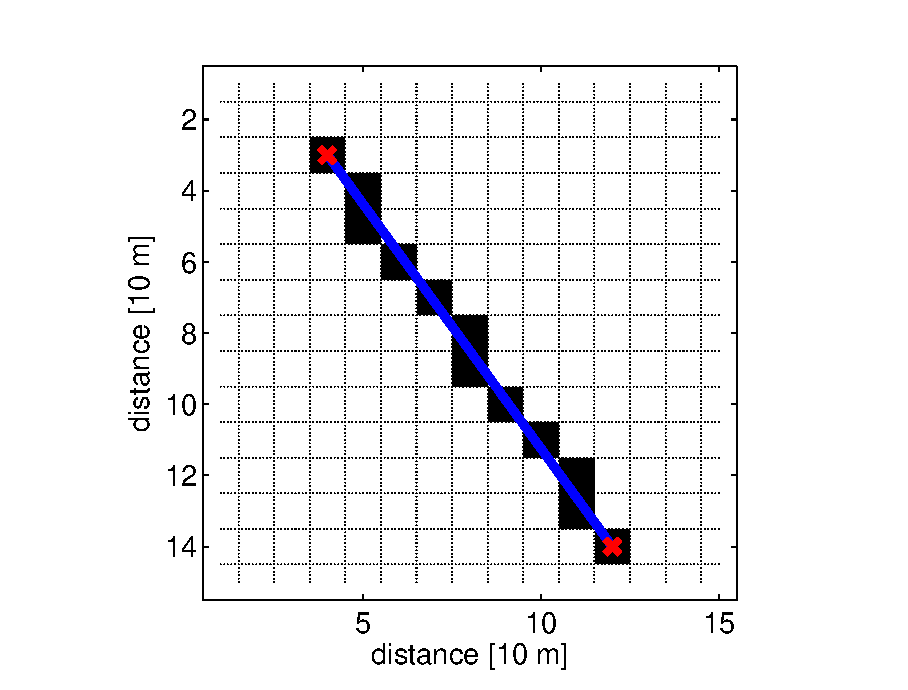
\includegraphics{data/bresenham.eps}}
			\caption{\textit{Example of Bresenham's line algorithm with map and path segment.}}
			\label{fig:bresenham}
		\end{figure}
		As the scout bees pass a distance of $v \cdot \Delta t_s$, respectively $\sqrt{(v_x \cdot \Delta t_s)^2 + (v_y \cdot \Delta t_s)^2}$ for a velocity $v$ and time step $\Delta t_s$ in every iteration step, multiple field are being passed at once. In order to check all fields between the last and current iteration step for flower patches, the Bresenham line algorithm is used. With this method, all integer coordinates between two given points on the map are reported back. Afterwards, every obtained point can be checked against the current quality- and type-map of the environment simulation.
		For this simple algorithm, a pre-existing implementation is used \cite{MVTB}, appendix \ref{chap:MATLAB_bresenham}. Figure \ref{fig:bresenham} is an example on a 15x15 map with coordinates $(x = 4, y = 3)$ to $(x = 12, y = 14)$ and reported points (black boxes).

\subsection{Foragers}
	\subsubsection{Path optimization}
		\label{chap:pathOptimization}
		
				\begin{figure}
					\centering
					\scalebox{.9}{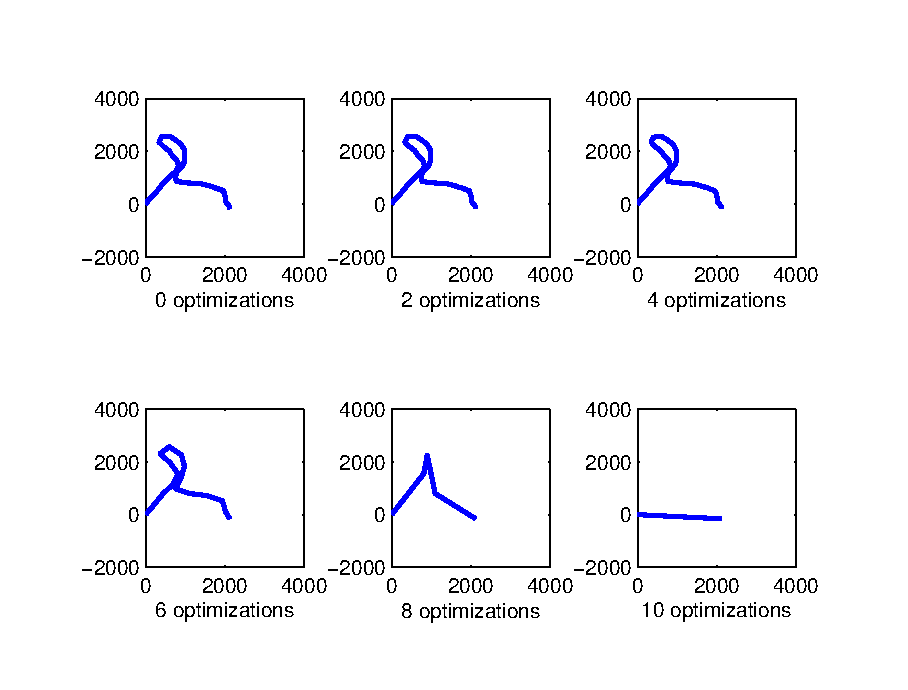
\includegraphics{data/optimization.eps}}
					\caption{\textit{Example of path optimization used to short cut the path to flower patches.}}
					\label{fig:pathOptimization}
				\end{figure}
		
		We assume bees can optimize the original path they obtain from a waggle dance, as the bees are able to orientate themselves in the environment with sun positioning \cite{seeley95}, p. 37. The implementation used is a simple one, in order to keep computation times low. At every point where optimization may occur (see chapter \ref{chap:beesWorkingStates}), there is a 50\% chance of optimization. Optimization works as follows:
		\[
			\begin{pmatrix}
				x_0 & x_1 & x_2 & x_3 & x_4 & \ldots & x_{n-3} & x_{n-2} & x_{n-1} & x_n \\
				y_0 & y_1 & y_2 & y_3 & y_4 & \ldots & y_{n-3} & y_{n-2} & y_{n-1} & y_n
			\end{pmatrix}
		\]
		\[
			\Longrightarrow_{optimization}
			\begin{pmatrix}
				x_0 & x_2 & x_4 & \ldots & x_{n-4} & x_{n-2} & x_{n} \\ y_0 & y_2 & y_4 & \ldots & y_{n-4} & y_{n-2} & y_{n}
			\end{pmatrix}
		\]
		This means every second way point is skipped, while starting- and endpoints are preserved. According to the triangle inequality, the $L^2$ norm of the distance can only become smaller after every such step, therefore it is an optimization in terms of path length. The outcome of such an optimization process on the path from Figure \ref{fig:randomWalk} is presented in Figure \ref{fig:pathOptimization}.\\
		Comparing this model of optimization with empirical observations made by \textit{Lihoreau et. al} \cite{lihoreau11}, p. 3, shows that our model is a good approximation: They state that the bees reduce their travel times gradually with experience and higher numbers of flights. The same happens with our model, as the shortest path is not taken directly, but shorter paths are taken after visiting a certain patch often enough. The only difference is that we don't explicitly simulate multi-patch sequences (bees can visit multiple patches before returning to the hive) while \textit{Lihoreau et. al} primarily focus on this matter.